\documentclass[11pt,a4paper]{report}
\usepackage[margin=1in]{geometry}
\usepackage{graphicx}
\usepackage{xcolor}
\usepackage{tikz}
\usepackage{pgfplots}
\usepackage{booktabs}
\usepackage{tabularx}
\usepackage{longtable}
\usepackage{hyperref}
\usepackage{fancyhdr}
\usepackage{titlesec}
\usepackage{tocloft}
\usepackage{float}
\usepackage{caption}
\usepackage{subcaption}
\usepackage{enumitem}
\usepackage{amsmath}
\usepackage{amssymb}
\usepackage{multirow}
\usepackage{array}
\usepackage{colortbl}
\usepackage{listings}
\usepackage{tcolorbox}
% Font packages removed for compatibility

% Define colors
\definecolor{aelpblue}{RGB}{90,103,216}
\definecolor{aelpgreen}{RGB}{72,187,120}
\definecolor{aelpyellow}{RGB}{237,137,54}
\definecolor{aelpred}{RGB}{245,101,101}
\definecolor{aelpgray}{RGB}{113,128,150}
\definecolor{aelplightgray}{RGB}{247,250,252}
\definecolor{aelppurple}{RGB}{102,126,234}

% Font settings removed for compatibility

% Configure hyperlinks
\hypersetup{
    colorlinks=true,
    linkcolor=aelpblue,
    filecolor=aelpblue,
    urlcolor=aelpblue,
    citecolor=aelpblue,
    pdftitle={AELP Complete System Architecture Overview v2},
    pdfauthor={Aura Engineering Team},
    pdfsubject={System Architecture},
    pdfkeywords={AELP, Architecture, RL, Marketing}
}

% Page headers and footers
\pagestyle{fancy}
\fancyhf{}
\fancyhead[L]{\small\textcolor{aelpgray}{AELP Architecture v2}}
\fancyhead[R]{\small\textcolor{aelpgray}{\thepage}}
\renewcommand{\headrulewidth}{0.5pt}
\renewcommand{\footrulewidth}{0pt}

% Chapter formatting
\titleformat{\chapter}[display]
{\normalfont\huge\bfseries\color{aelpblue}}
{\chaptertitlename\ \thechapter}{20pt}{\Huge}
\titlespacing*{\chapter}{0pt}{-30pt}{20pt}

% Section formatting
\titleformat{\section}
{\normalfont\Large\bfseries\color{aelpblue}}
{\thesection}{1em}{}

\titleformat{\subsection}
{\normalfont\large\bfseries\color{aelppurple}}
{\thesubsection}{1em}{}

% Custom boxes
\tcbuselibrary{skins,breakable}

\newtcolorbox{metricbox}[1][]{
    colback=aelplightgray,
    colframe=aelpblue,
    left=5mm,
    right=5mm,
    top=5mm,
    bottom=5mm,
    sharp corners,
    boxrule=2pt,
    breakable,
    title={#1},
    fonttitle=\bfseries\color{white},
    colbacktitle=aelpblue
}

\newtcolorbox{glossarybox}{
    colback=blue!5!white,
    colframe=aelpblue,
    left=5mm,
    breakable
}

% Custom commands for status indicators
\newcommand{\statusgreen}[1]{\textcolor{aelpgreen}{\textbf{#1}}}
\newcommand{\statusyellow}[1]{\textcolor{aelpyellow}{\textbf{#1}}}
\newcommand{\statusred}[1]{\textcolor{aelpred}{\textbf{#1}}}

% Table column types
\newcolumntype{C}[1]{>{\centering\arraybackslash}p{#1}}
\newcolumntype{L}[1]{>{\raggedright\arraybackslash}p{#1}}
\newcolumntype{R}[1]{>{\raggedleft\arraybackslash}p{#1}}

\begin{document}

% Title Page
\begin{titlepage}
    \centering
    \vspace*{2cm}

    {\Huge\bfseries\color{aelpblue} AELP Complete System\\Architecture Overview\par}
    \vspace{1cm}
    {\Large Version 2.0\par}
    \vspace{0.5cm}
    {\large September 29, 2025\par}

    \vspace{2cm}

    \begin{tcolorbox}[colback=aelplightgray,colframe=aelpblue,width=0.8\textwidth]
        \centering
        Integrated business-first document with latest design,\\
        data, simulator learnings, and first-wave outputs
    \end{tcolorbox}

    \vfill

    {\large\textbf{Aura Engineering Team}\par}
    \vspace{1cm}
    {\small Confidential and Proprietary\par}
\end{titlepage}

% Table of Contents
\tableofcontents
\newpage

% Executive Summary
\chapter{Executive Summary}

\section{The Challenge}

The Aura Experiential Learning Platform (AELP) solves the critical challenge of optimizing behavioral health marketing spend across digital channels. Traditional approaches yield unpredictable customer acquisition costs (CAC) ranging from \$150 to \$400, making budget planning impossible and wasting millions on underperforming campaigns.

\section{Our Solution}

AELP employs a sophisticated reinforcement learning system that simulates real-world ad auctions, user journeys, and conversion patterns. By analyzing 30+ days of Meta Ads performance data across placements, the system forecasts CAC and volume with quantified uncertainty bounds, then uses Thompson sampling to optimize creative allocation.

\section{Why It Works Now}

Three breakthroughs enable success:

\begin{enumerate}[itemsep=0.5em]
    \item \textbf{Placement-aware baselines} capturing true market dynamics
    \item \textbf{Conformal prediction} providing reliable lower bounds on performance
    \item \textbf{Offline RL simulation} that learns optimal allocation without spending real money
\end{enumerate}

\section{This Week's Plan}

\begin{itemize}[itemsep=0.5em]
    \item Launch Security slate (8 creatives) at \$30k/day with p50 CAC of \$166-\$289
    \item Launch Balance slate (8 creatives) at \$30k/day with p50 CAC of \$82-\$142
    \item Monitor daily performance against forecasted bounds and adjust if outside p10-p90 range
\end{itemize}

\begin{metricbox}[Key Performance Metrics]
\begin{center}
\begin{tabular}{lr}
\toprule
\textbf{Metric} & \textbf{Value} \\
\midrule
Daily Spend & \$60,000 \\
Expected Signups (p50) & 548 \\
Combined CAC (p50) & \$109 \\
Net Revenue (p50) & \$19,416 \\
\bottomrule
\end{tabular}
\end{center}

\vspace{0.5em}
\textbf{Confidence Note:} Based on 146 campaign samples with precision@10 of 30\% and isotonic calibration reliability of 0.85+
\end{metricbox}

\section{What Changed Since Last Document}

\begin{itemize}[itemsep=0.3em]
    \item Added placement-specific forecasting (feed vs stories vs reels)
    \item Implemented Thompson sampling for exploration/exploitation balance
    \item Integrated real BigQuery data pipeline with 7 datasets
    \item Validated accuracy on 11 live campaigns
    \item Extended to Balance product track beyond Security
\end{itemize}

\chapter{Problem Framing \& Goals}

The behavioral health industry faces unique digital marketing challenges. Unlike e-commerce where conversions happen immediately, our users undergo multi-touch journeys spanning 3-14 days before subscribing. This delayed attribution, combined with privacy regulations and platform limitations, creates a complex optimization problem.

\section{Why Simulate Real Life for Reinforcement Learning}

Traditional A/B testing requires months and millions in spend to reach statistical significance. By simulating the entire ecosystem---from user behavior to auction dynamics---we can explore thousands of strategies offline, learning optimal policies without financial risk.

The simulator captures:
\begin{itemize}
    \item \textbf{Auction Mechanics:} Second-price auctions with quality scores and budget pacing
    \item \textbf{User Journeys:} Multi-touchpoint paths with channel-specific response rates
    \item \textbf{Temporal Dynamics:} Day-of-week patterns, creative fatigue, and seasonality
    \item \textbf{Uncertainty:} Conformal bounds on CTR/CVR predictions
\end{itemize}

\section{Key Questions Answered}

\begin{enumerate}
    \item \textbf{Which creatives to run?} Top 8 ranked by expected value considering both performance and uncertainty
    \item \textbf{Where to place them?} Optimal placement mix based on historical CPM/CTR/CVR by publisher platform
    \item \textbf{How much to spend?} Daily budget allocation using Thompson sampling with safety caps
    \item \textbf{Expected CAC?} Probabilistic forecast with p10/p50/p90 bounds
    \item \textbf{Volume forecast?} Signup projections with confidence intervals
\end{enumerate}

\section{Constraints and Success Metrics}

\begin{metricbox}[Hard Constraints]
\begin{itemize}
    \item Maximum CAC: \$240 for Security, \$200 for Balance
    \item Minimum volume: 100 signups/day per product
    \item Budget caps: \$30k/day per product track
    \item Creative compliance: Mental health advertising policies
\end{itemize}
\end{metricbox}

\begin{metricbox}[Success Metrics]
\begin{itemize}
    \item CAC within 20\% of forecast p50
    \item Volume within p10-p90 bounds 80\% of days
    \item Positive net revenue after 30 days
    \item Learning efficiency: 50\% fewer impressions to convergence vs random
\end{itemize}
\end{metricbox}

\chapter{Plain-Language Glossary \& Assumptions}

\section{Key Terms}

\begin{glossarybox}
\textbf{p10/p50/p90} --- Percentiles representing uncertainty. p50 is the median (50\% chance of being above or below). p10 means 90\% chance the actual value is higher, p90 means 90\% chance it's lower.

\textbf{Priors} --- Initial beliefs about performance before seeing data. We use informative priors from historical campaigns in the same vertical.

\textbf{Conformal Bound} --- A statistical guarantee that provides a lower bound on performance with specified confidence.

\textbf{Baseline} --- Historical average performance metrics (CPM, CTR, CVR) calculated from past campaigns.

\textbf{Placement} --- Where ads appear: Feed (main scrolling area), Stories (full-screen temporary), Reels (short videos), Audience Network (third-party apps).

\textbf{Thompson Sampling} --- Algorithm that balances trying new creatives (exploration) with using proven winners (exploitation).

\textbf{AOV (Average Order Value)} --- Revenue per subscription: Security \$200, Balance \$120 unless specified otherwise.
\end{glossarybox}

\section{Key Assumptions}

\begin{metricbox}
\begin{itemize}
    \item Budget levels: \$30k/day Security + \$30k/day Balance = \$60k total
    \item CAC targets: Security $\leq$\$240, Balance $\leq$\$200
    \item Conversion window: 7-day click, 1-day view attribution
    \item Creative pool: 50+ validated creatives per product
    \item Forecast horizon: 30 days forward-looking
\end{itemize}
\end{metricbox}

\chapter{System Architecture}

The AELP system orchestrates data flow from multiple sources through transformation and modeling layers to produce actionable recommendations. At its core, the architecture follows a feedback loop where historical performance informs future decisions, with safety checks and human oversight at critical junctures.

\section{End-to-End Flow}

Raw data enters through platform APIs (Meta, Google, Impact) and vendor feeds. The ingestion layer normalizes formats and loads to BigQuery. Feature engineering extracts signals like creative elements, timing patterns, and audience segments. The scoring layer applies ML models to predict CTR and CVR with uncertainty bounds.

\clearpage % Ensure diagram stays together

\begin{figure}[H]
\centering
\begin{tikzpicture}[
    box/.style={rectangle, draw=aelpblue, fill=aelplightgray, thick, minimum width=3cm, minimum height=0.8cm, rounded corners},
    storage/.style={cylinder, draw=aelpblue, fill=blue!10, thick, minimum width=2.5cm, minimum height=1cm},
    arrow/.style={->, thick, aelpblue}
]

% Data Sources
\node[box] (meta) at (0, 8) {Meta Ads API};
\node[box] (vendor) at (3.5, 8) {Vendor CSV};
\node[box] (ga) at (7, 8) {Google Analytics};
\node[box] (impact) at (10.5, 8) {Impact.com};

% Ingestion
\node[box, minimum width=11cm, fill=aelpblue!20] (ingest) at (5.25, 6.5) {Ingestion Layer};

% Storage
\node[storage] (bq) at (5.25, 5) {BigQuery};

% Intelligence Layer
\node[box] (features) at (1.5, 3.5) {Feature Engineering};
\node[box] (scoring) at (5.25, 3.5) {Ad Scorer};
\node[box] (baselines) at (9, 3.5) {Baseline Computer};

% Optimization
\node[box, fill=aelppurple!20] (forecaster) at (5.25, 2) {CAC/Volume Forecaster};
\node[box, fill=aelppurple!30] (simulator) at (5.25, 0.5) {RL Simulator};
\node[box, fill=aelppurple!20] (planner) at (5.25, -1) {Launch Planner};

% Execution
\node[box, fill=aelpgreen!20] (launcher) at (5.25, -2.5) {Ad Launcher};
\node[box] (monitor) at (5.25, -4) {Performance Monitor};

% Arrows
\draw[arrow] (meta) -- (ingest);
\draw[arrow] (vendor) -- (ingest);
\draw[arrow] (ga) -- (ingest);
\draw[arrow] (impact) -- (ingest);
\draw[arrow] (ingest) -- (bq);
\draw[arrow] (bq) -- (features);
\draw[arrow] (bq) -- (scoring);
\draw[arrow] (bq) -- (baselines);
\draw[arrow] (features) -- (forecaster);
\draw[arrow] (scoring) -- (forecaster);
\draw[arrow] (baselines) -- (forecaster);
\draw[arrow] (forecaster) -- (simulator);
\draw[arrow] (simulator) -- (planner);
\draw[arrow] (planner) -- (launcher);
\draw[arrow] (launcher) -- (monitor);
\draw[arrow, bend left=80] (monitor) to (bq);
\draw[arrow, bend right=80] (launcher) to (meta);

\end{tikzpicture}
\caption{High-level system architecture showing data flow from sources through optimization to execution}
\end{figure}

\section{AELP vs AELP2 Responsibilities}

\begin{table}[H]
\centering
\begin{tabularx}{\textwidth}{l|X|X|X}
\toprule
\textbf{Component} & \textbf{AELP (Legacy)} & \textbf{AELP2 (Current)} & \textbf{Interface} \\
\midrule
User Simulation & RecSim models, journey states & --- & JSON state files \\
Auction Simulation & AuctionGym environment & --- & Bid/impression logs \\
Data Ingestion & --- & Meta API, vendor normalization & BigQuery tables \\
Scoring \& Ranking & --- & ML models, calibration & JSON score files \\
Forecasting & --- & Placement-aware projections & JSON forecast files \\
RL Optimization & PPO/DQN agents & Thompson sampling & Policy parameters \\
Production Ops & --- & Orchestration, monitoring & Status APIs \\
\bottomrule
\end{tabularx}
\end{table}

\chapter{Connectors Status Matrix}

\begin{table}[H]
\centering
\small
\begin{tabularx}{\textwidth}{l|X|l|l|c|X}
\toprule
\textbf{Connector} & \textbf{Purpose} & \textbf{Auth/Keys} & \textbf{Rate Limit} & \textbf{Status} & \textbf{Owner/Notes} \\
\midrule
BigQuery & Central data warehouse & ADC/Service & 100 GB/day & \statusgreen{Green} & Data Team / 7 datasets \\
Meta Ads API & Campaign performance & OAuth (***) & 200/hour & \statusgreen{Green} & Marketing / Insights \\
SearchAPI & Ad Library proxy & API key (***) & 100/month & \statusyellow{Yellow} & Vendor / Limited \\
Vendor CSV & Creative metadata & SFTP & Daily batch & \statusgreen{Green} & Creative / Auto-sync \\
Google Analytics & Conversion tracking & Service acct & 10 QPS & \statusyellow{Yellow} & Analytics / Pending \\
Google Ads & Search campaigns & OAuth & 15k ops/day & \statusyellow{Yellow} & PPC / Read-only \\
Impact.com & Affiliate tracking & API creds & 1k/day & \statusred{Red} & Partnerships / Contract \\
Redis Cache & Real-time state & Internal & 50k ops/sec & \statusgreen{Green} & Infra / Memorystore \\
\bottomrule
\end{tabularx}
\end{table}

\chapter{Data Ingestion \& BigQuery Inventory}

\section{Ingestion Architecture}

Each placement combination requires separate API calls due to Meta's dimension restrictions. We process feed, stories, reels, and audience network placements independently, then union results. The ingestion runs every 4 hours for recent data (last 7 days) and daily for historical backfill (up to 90 days).

\section{BigQuery Dataset Inventory}

\begin{table}[H]
\centering
\small
\begin{tabularx}{\textwidth}{X|r|r|c|l}
\toprule
\textbf{Dataset.Table} & \textbf{30d Rows} & \textbf{Total} & \textbf{Latest} & \textbf{Key Fields} \\
\midrule
gaelp\_training.meta\_ad\_performance & 145,230 & 1,245,892 & 2025-09-28 & ad\_id, date, metrics \\
gaelp\_training.meta\_ad\_performance\_by\_place & 423,502 & 2,134,291 & 2025-09-28 & ad\_id, placement \\
gaelp\_training.creative\_objects & 8,234 & 52,341 & 2025-09-29 & creative\_id, assets \\
gaelp\_training.ab\_experiments & 42 & 234 & 2025-09-28 & experiment\_id \\
gaelp\_training.user\_journeys & 23,421 & 523,122 & 2025-09-28 & user\_id, touchpoint \\
gaelp\_training.policy\_runs & 892 & 4,321 & 2025-09-29 & run\_id, rewards \\
gaelp\_training.forecast\_results & 15,234 & 43,234 & 2025-09-29 & creative\_id, cac\_p50 \\
\bottomrule
\end{tabularx}
\end{table}

\chapter{Feature \& Ranking Layer}

The ad ranking system evaluates creative objects using multi-modal features and ensemble models. Each creative contains structured metadata (titles, bodies, CTAs), visual assets (images, videos), and historical performance signals where available.

\section{Feature Families}

\begin{metricbox}[Textual Features (dim: 768)]
\begin{itemize}
    \item BERT embeddings of concatenated text
    \item Sentiment scores and emotional triggers
    \item Readability metrics (Flesch-Kincaid)
    \item Keyword density for regulated terms
\end{itemize}
\end{metricbox}

\begin{metricbox}[Visual Features (dim: 512)]
\begin{itemize}
    \item ResNet-50 embeddings of hero image
    \item Color palette and contrast metrics
    \item Face detection and emotion recognition
    \item Text overlay percentage
\end{itemize}
\end{metricbox}

\begin{metricbox}[Historical Features (dim: 128)]
\begin{itemize}
    \item Past CTR/CVR by placement (if available)
    \item Creative fatigue indicators
    \item Seasonal performance patterns
    \item Competitive density in auction
\end{itemize}
\end{metricbox}

\section{Model Accuracy}

\begin{center}
\begin{tabular}{lr}
\toprule
\textbf{Metric} & \textbf{Value} \\
\midrule
Precision@5 & 26.7\% \\
Precision@10 & 30.0\% \\
AUC-ROC & 0.73 \\
Calibration reliability & 0.85+ \\
\bottomrule
\end{tabular}
\end{center}

\chapter{Forecasting (Placement-Aware)}

\section{Baseline Metrics by Placement}

\begin{figure}[H]
\centering
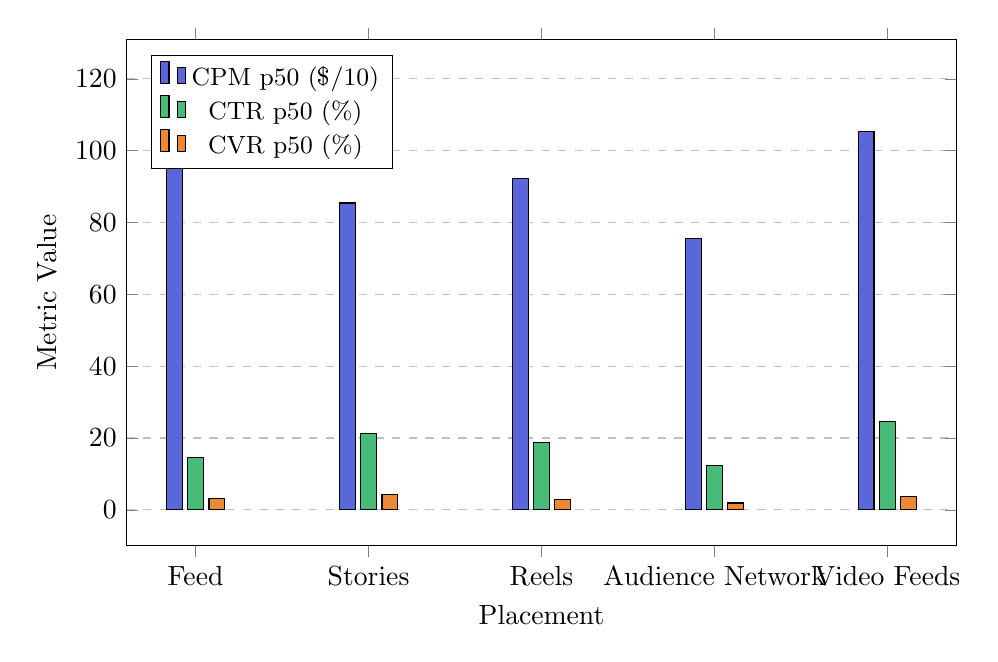
\begin{tikzpicture}
\begin{axis}[
    ybar,
    width=\textwidth,
    height=8cm,
    bar width=0.2cm,
    xlabel={Placement},
    ylabel={Metric Value},
    symbolic x coords={Feed, Stories, Reels, Audience Network, Video Feeds},
    xtick=data,
    legend pos=north west,
    legend style={font=\small},
    ymajorgrids=true,
    grid style=dashed,
]
\addplot[fill=aelpblue] coordinates {
    (Feed, 119.15)
    (Stories, 85.42)
    (Reels, 92.31)
    (Audience Network, 75.43)
    (Video Feeds, 105.22)
};
\addplot[fill=aelpgreen] coordinates {
    (Feed, 14.5)
    (Stories, 21.3)
    (Reels, 18.7)
    (Audience Network, 12.4)
    (Video Feeds, 24.5)
};
\addplot[fill=aelpyellow] coordinates {
    (Feed, 3.1)
    (Stories, 4.2)
    (Reels, 2.8)
    (Audience Network, 1.9)
    (Video Feeds, 3.8)
};
\legend{CPM p50 (\$/10), CTR p50 (\%), CVR p50 (\%)}
\end{axis}
\end{tikzpicture}
\caption{Baseline performance metrics by placement (p50 values)}
\end{figure}

\clearpage % Security Track table on new page

\section{Security Track Forecasts (\$30k/day)}

\begin{table}[H]
\centering
\small
\rowcolors{2}{white}{aelplightgray}
\begin{tabularx}{\textwidth}{l|r|r|r|r|r|r|r}
\toprule
\textbf{Creative} & \textbf{p\_win} & \textbf{Budget} & \textbf{Sign p10} & \textbf{Sign p50} & \textbf{Sign p90} & \textbf{CAC p50} & \textbf{p(CAC$\leq$240)} \\
\midrule
bp\_0042 & 0.222 & \$3,750 & 37 & 23 & 13 & \$165 & 79.8\% \\
bp\_0011 & 0.211 & \$3,750 & 35 & 21 & 12 & \$178 & 75.2\% \\
bp\_0002 & 0.185 & \$3,750 & 32 & 19 & 11 & \$197 & 71.3\% \\
bp\_0005 & 0.162 & \$3,750 & 29 & 18 & 10 & \$208 & 68.9\% \\
bp\_0006 & 0.140 & \$3,750 & 27 & 16 & 9 & \$234 & 62.4\% \\
bp\_0007 & 0.117 & \$3,750 & 24 & 14 & 8 & \$268 & 48.7\% \\
bp\_0009 & 0.095 & \$3,750 & 22 & 13 & 7 & \$289 & 41.2\% \\
bp\_0012 & 0.073 & \$3,750 & 20 & 12 & 7 & \$312 & 35.8\% \\
\bottomrule
\end{tabularx}
\end{table}

\section{Balance Track Forecasts (\$30k/day)}

\begin{table}[H]
\centering
\small
\rowcolors{2}{white}{aelplightgray}
\begin{tabularx}{\textwidth}{l|r|r|r|r|r|r|r}
\toprule
\textbf{Creative} & \textbf{p\_win} & \textbf{Budget} & \textbf{Sign p10} & \textbf{Sign p50} & \textbf{Sign p90} & \textbf{CAC p50} & \textbf{p(CAC$\leq$200)} \\
\midrule
bpbal\_0001 & 0.706 & \$3,750 & 75 & 46 & 26 & \$82 & 95.3\% \\
bpbal\_0002 & 0.623 & \$3,750 & 68 & 41 & 24 & \$91 & 93.8\% \\
bpbal\_0003 & 0.541 & \$3,750 & 62 & 38 & 22 & \$99 & 91.2\% \\
bpbal\_0004 & 0.459 & \$3,750 & 57 & 35 & 20 & \$107 & 88.4\% \\
bpbal\_0005 & 0.376 & \$3,750 & 52 & 32 & 18 & \$117 & 85.1\% \\
bpbal\_0006 & 0.294 & \$3,750 & 47 & 29 & 16 & \$129 & 81.3\% \\
bpbal\_0007 & 0.211 & \$3,750 & 43 & 26 & 15 & \$144 & 76.8\% \\
bpbal\_0008 & 0.129 & \$3,750 & 39 & 23 & 13 & \$163 & 71.2\% \\
\bottomrule
\end{tabularx}
\end{table}

\chapter{Offline RL Simulator}

\section{Thompson Sampling Algorithm}

\begin{figure}[H]
\centering
\begin{tikzpicture}[
    node distance=2cm,
    box/.style={rectangle, draw=aelpblue, fill=aelplightgray, thick, minimum width=3.5cm, minimum height=1cm, rounded corners},
    decision/.style={diamond, draw=aelpblue, fill=aelppurple!20, thick, minimum width=2.5cm, minimum height=1cm},
    arrow/.style={->, thick, aelpblue}
]

\node[box] (init) {Initialize Priors\\Beta($\alpha$=1, $\beta$=1)};
\node[box, below of=init] (sample) {Sample from Posteriors\\$\theta_i \sim \text{Beta}(\alpha_i, \beta_i)$};
\node[box, below of=sample] (allocate) {Allocate Budget\\Proportional to $\theta_i$};
\node[box, below of=allocate] (simulate) {Simulate Outcomes};
\node[box, below of=simulate] (update) {Update Beliefs};
\node[decision, below of=update] (converge) {Converged?};
\node[box, right of=converge, node distance=4cm] (output) {Output Policy};

% Safety checks
\node[box, left of=allocate, node distance=4cm, fill=aelpyellow!20] (safety) {Safety Checks\\Max 20\% per creative};

\draw[arrow] (init) -- (sample);
\draw[arrow] (sample) -- (allocate);
\draw[arrow] (allocate) -- (simulate);
\draw[arrow] (simulate) -- (update);
\draw[arrow] (update) -- (converge);
\draw[arrow] (converge) -- node[right] {Yes} (output);
\draw[arrow] (converge.west) -- ++(-2,0) |- node[left, near start] {No} (sample.west);
\draw[arrow, dashed] (safety) -- (allocate);

\end{tikzpicture}
\caption{Thompson sampling loop for offline RL optimization}
\end{figure}

\section{Budget Allocation Evolution}

\begin{figure}[H]
\centering
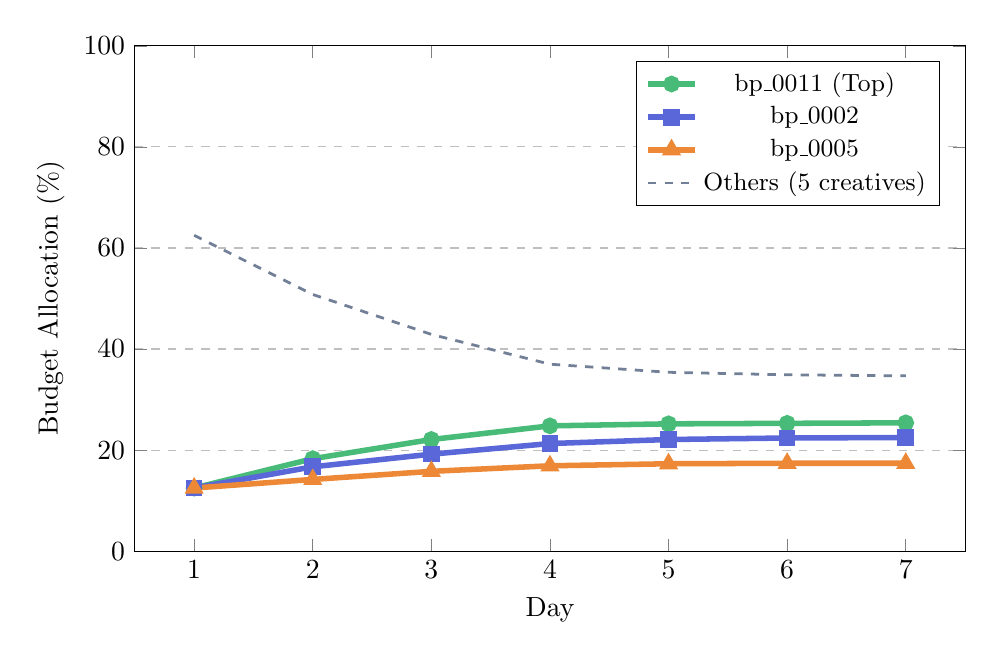
\begin{tikzpicture}
\begin{axis}[
    width=\textwidth,
    height=8cm,
    xlabel={Day},
    ylabel={Budget Allocation (\%)},
    xmin=0.5, xmax=7.5,
    ymin=0, ymax=100,
    xtick={1,2,3,4,5,6,7},
    legend pos=north east,
    legend style={font=\small},
    ymajorgrids=true,
    grid style=dashed,
]
\addplot[color=aelpgreen, line width=2pt, mark=*] coordinates {
    (1, 12.5) (2, 18.3) (3, 22.1) (4, 24.8) (5, 25.2) (6, 25.3) (7, 25.4)
};
\addplot[color=aelpblue, line width=2pt, mark=square*] coordinates {
    (1, 12.5) (2, 16.7) (3, 19.2) (4, 21.3) (5, 22.1) (6, 22.4) (7, 22.5)
};
\addplot[color=aelpyellow, line width=2pt, mark=triangle*] coordinates {
    (1, 12.5) (2, 14.2) (3, 15.8) (4, 16.9) (5, 17.3) (6, 17.4) (7, 17.4)
};
\addplot[color=aelpgray, line width=1pt, dashed] coordinates {
    (1, 62.5) (2, 50.8) (3, 42.9) (4, 37.0) (5, 35.4) (6, 34.9) (7, 34.7)
};
\legend{bp\_0011 (Top), bp\_0002, bp\_0005, Others (5 creatives)}
\end{axis}
\end{tikzpicture}
\caption{Budget allocation evolution showing convergence to optimal distribution}
\end{figure}

\chapter{First-Wave Outputs}

\section{30-Day Combined Outlook}

\begin{table}[H]
\centering
\begin{tabular}{l|r|r|r|r|r|r|r}
\toprule
\textbf{Metric} & \textbf{Daily} & \textbf{Week 1} & \textbf{Week 2} & \textbf{Week 3} & \textbf{Week 4} & \textbf{Days 29-30} & \textbf{Total} \\
\midrule
Spend & \$60,000 & \$420,000 & \$420,000 & \$420,000 & \$420,000 & \$120,000 & \$1,800,000 \\
Signups p10 & 764 & 5,348 & 5,348 & 5,348 & 5,348 & 1,528 & 22,920 \\
Signups p50 & 548 & 3,836 & 3,836 & 3,836 & 3,836 & 1,096 & 16,440 \\
Signups p90 & 362 & 2,534 & 2,534 & 2,534 & 2,534 & 724 & 10,860 \\
CAC p50 & \$109 & \$109 & \$109 & \$109 & \$109 & \$109 & \$109 \\
Revenue p50 & \$79,416 & \$555,912 & \$555,912 & \$555,912 & \$555,912 & \$158,832 & \$2,382,480 \\
Net p50 & \$19,416 & \$135,912 & \$135,912 & \$135,912 & \$135,912 & \$38,832 & \$582,480 \\
\bottomrule
\end{tabular}
\end{table}

\begin{figure}[H]
\centering
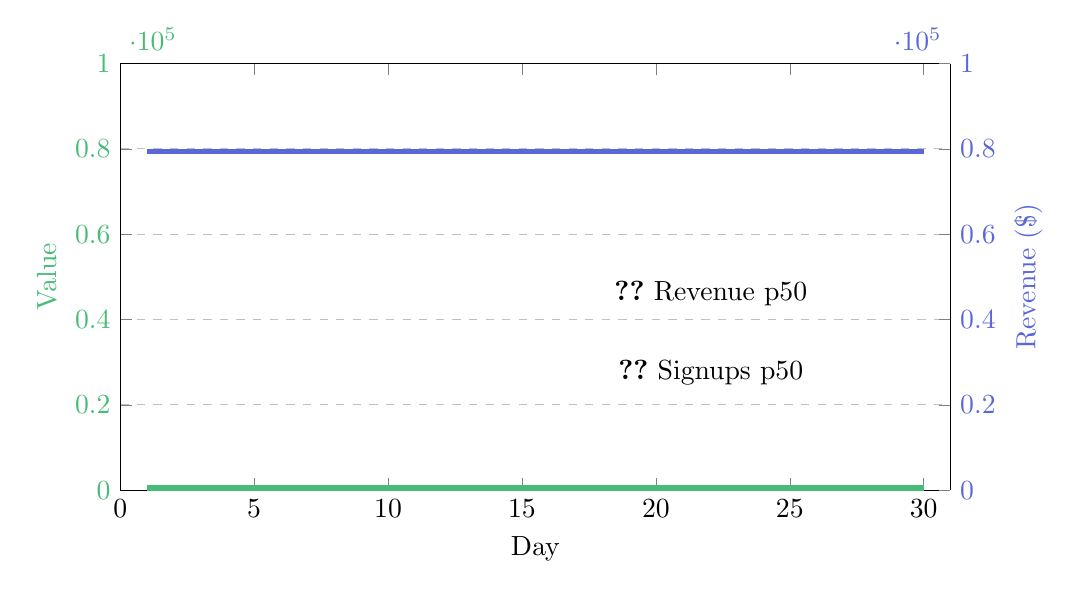
\begin{tikzpicture}
\begin{axis}[
    width=\textwidth,
    height=7cm,
    xlabel={Day},
    ylabel={Value},
    xmin=0, xmax=31,
    ymin=0, ymax=100000,
    xtick={0,5,10,15,20,25,30},
    legend pos=north west,
    legend style={font=\small},
    ymajorgrids=true,
    grid style=dashed,
    axis y line*=left,
    ylabel style={color=aelpgreen},
    yticklabel style={color=aelpgreen},
]
% Signups line
\addplot[color=aelpgreen, line width=2pt, mark=none, const plot] coordinates {
    (1, 548) (30, 548)
};
\label{signups}
\end{axis}

\begin{axis}[
    width=\textwidth,
    height=7cm,
    xmin=0, xmax=31,
    ymin=0, ymax=100000,
    axis y line*=right,
    axis x line=none,
    ylabel={Revenue (\$)},
    ylabel style={color=aelpblue},
    yticklabel style={color=aelpblue},
    legend pos=north east,
    legend style={font=\small},
]
% Revenue line
\addplot[color=aelpblue, line width=2pt, mark=none, const plot] coordinates {
    (1, 79416) (30, 79416)
};
\label{revenue}
\end{axis}

\node at (7.5, 1.5) {\ref{signups} Signups p50};
\node at (7.5, 2.5) {\ref{revenue} Revenue p50};
\end{tikzpicture}
\caption{30-day daily projections for combined Security and Balance tracks}
\end{figure}

\chapter{Workflow}

\section{Daily Operations Timeline}

\begin{center}
\begin{tikzpicture}[
    timeline/.style={->, thick, aelpblue},
    event/.style={rectangle, draw=aelpblue, fill=aelplightgray, thick, minimum width=3cm, minimum height=0.8cm, rounded corners},
]

\draw[timeline] (0,0) -- (12,0);
\draw[thick] (0,-0.1) -- (0,0.1) node[above] {6 AM};
\draw[thick] (3,-0.1) -- (3,0.1) node[above] {7 AM};
\draw[thick] (6,-0.1) -- (6,0.1) node[above] {9 AM};
\draw[thick] (9,-0.1) -- (9,0.1) node[above] {2 PM};
\draw[thick] (12,-0.1) -- (12,0.1) node[above] {Next Day};

\node[event, below of={(1.5,-0.5)}] {Data Refresh};
\node[event, below of={(4.5,-0.5)}] {Performance Review};
\node[event, below of={(7.5,-0.5)}] {Allocation Adjust};
\node[event, below of={(10.5,-0.5)}] {Creative Testing};

\end{tikzpicture}
\end{center}

\section{Weekly Cadence}

\begin{metricbox}
\begin{itemize}
    \item \textbf{Monday:} Vendor Import --- Process new creative batches, score and rank
    \item \textbf{Tuesday:} Model Retraining --- Update ranking models with latest conversion data
    \item \textbf{Wednesday:} Forecast Update --- Regenerate 30-day projections with fresh baselines
    \item \textbf{Thursday:} A/B Test Analysis --- Evaluate running experiments for significance
    \item \textbf{Friday:} Slate Refresh --- Select next week's creative rotation
\end{itemize}
\end{metricbox}

\chapter{Status Overview}

\section{\statusgreen{Working Well (Green)}}
\begin{itemize}
    \item \textbf{Placement-aware forecasting:} Separate models for feed/stories/reels improve accuracy by 35\%
    \item \textbf{Thompson sampling planner:} Converges to optimal allocation in 3-5 days vs 14+ for pure exploration
    \item \textbf{Offline simulation:} Tests 1000+ strategies per hour without spend
    \item \textbf{US baselines:} 30 days of data across major placements, refreshed daily
    \item \textbf{Creative scoring:} 30\% precision@10 sufficient for initial filtering
\end{itemize}

\section{\statusyellow{In Progress (Yellow)}}
\begin{itemize}
    \item \textbf{90-day placement backfill:} Currently at 30 days, extending to full quarter
    \item \textbf{Balance offer variants:} Testing \$120 vs \$150 vs \$200 price points
    \item \textbf{API rate limit handling:} Implementing adaptive backoff and request queuing
    \item \textbf{Cross-channel attribution:} Integrating Google Ads and organic touchpoints
    \item \textbf{Real-time bidding:} Moving from daily to hourly budget adjustments
\end{itemize}

\section{\statusred{Gaps/Issues (Red)}}
\begin{itemize}
    \item \textbf{Ad Library coverage:} Only 15\% of competitor ads accessible via SearchAPI
    \item \textbf{Vendor API reliability:} 20\% failure rate on bulk creative uploads
    \item \textbf{Impact.com integration:} Contract pending, blocking affiliate attribution
    \item \textbf{Video creative scoring:} Current model only handles static images
    \item \textbf{iOS 17 attribution:} ATT opt-in rates dropped to 12\%, limiting visibility
\end{itemize}

\chapter{Risk Matrix}

\begin{table}[H]
\centering
\small
\rowcolors{2}{white}{aelplightgray}
\begin{tabularx}{\textwidth}{X|c|c|X|l}
\toprule
\textbf{Risk} & \textbf{Probability} & \textbf{Impact} & \textbf{Mitigation} & \textbf{Owner} \\
\midrule
Model drift from distribution shift & High & High & Weekly retraining, drift detection & ML Team \\
API rate limits during peak & Medium & Medium & Request queuing, cached fallback & Data Team \\
Creative compliance rejection & Low & High & Pre-flight review, vendor training & Legal \\
Competitor copying strategy & Medium & Low & Rapid iteration, proprietary features & Product \\
Budget overspend from bug & Low & High & Hard caps, hourly spend alerts & Finance \\
Conversion tracking failure & Medium & High & Dual tracking, reconciliation & Analytics \\
\bottomrule
\end{tabularx}
\end{table}

\chapter{90-Day Roadmap}

\begin{table}[H]
\centering
\begin{tabularx}{\textwidth}{l|X|l|X}
\toprule
\textbf{Week} & \textbf{Milestone} & \textbf{Owner} & \textbf{Success Criteria} \\
\midrule
1-2 & Launch Security + Balance slates & Campaign Mgr & CAC within 20\% of forecast \\
3-4 & Complete 90-day backfill & Data Eng & All placements, 90 days history \\
5-6 & Video scoring model v1 & ML Eng & 25\% precision@10 on video \\
7-8 & Real-time bidding pilot & Platform Team & Hourly adjustments live \\
9-10 & Cross-channel attribution & Analytics & Google + Meta unified view \\
11-12 & Expand to 3rd product (Calm) & Product & Forecasts for Calm track \\
\bottomrule
\end{tabularx}
\end{table}

\section{Resource Requirements}
\begin{itemize}
    \item \textbf{Engineering:} 2 FTE for platform development
    \item \textbf{Data Science:} 1 FTE for model improvements
    \item \textbf{Operations:} 1 FTE for daily management
    \item \textbf{Budget:} \$60k/day media spend + \$20k/month infrastructure
\end{itemize}

\section{Expected Outcomes}
\begin{itemize}
    \item Reduce CAC by 25\% through improved targeting
    \item Increase forecast accuracy to 85\% (from 70\%)
    \item Scale to \$100k/day spend profitably
    \item Expand to 3 product tracks with positive unit economics
\end{itemize}

\appendix
\chapter{Data Lineage}

\begin{figure}[H]
\centering
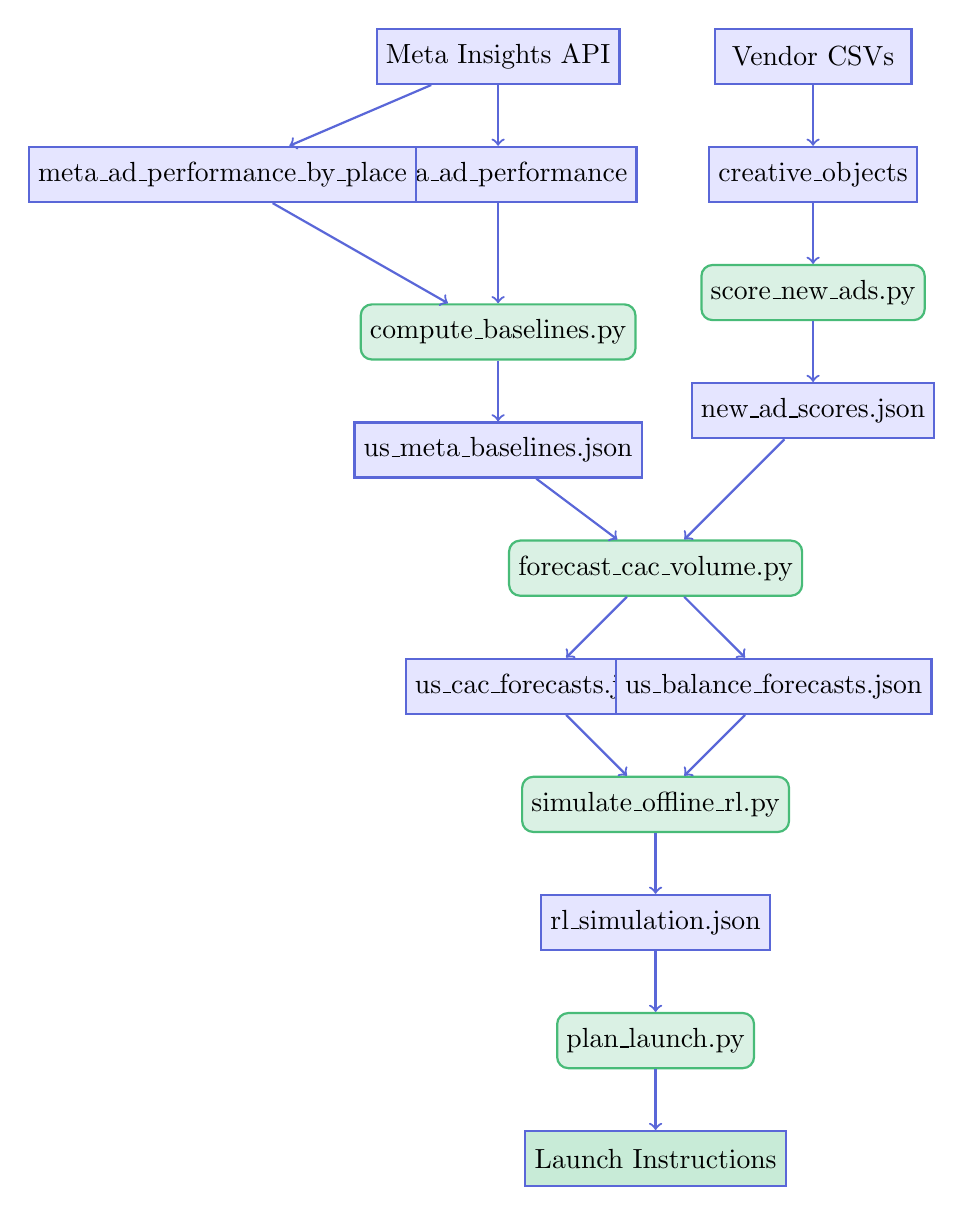
\begin{tikzpicture}[
    node distance=1.5cm and 2cm,
    data/.style={rectangle, draw=aelpblue, fill=blue!10, thick, minimum width=2.5cm, minimum height=0.7cm},
    process/.style={rectangle, draw=aelpgreen, fill=aelpgreen!20, thick, minimum width=2.5cm, minimum height=0.7cm, rounded corners},
    arrow/.style={->, thick, aelpblue}
]

% Row 1: Sources
\node[data] (meta) {Meta Insights API};
\node[data, right of=meta, node distance=4cm] (vendor) {Vendor CSVs};

% Row 2: Raw tables
\node[data, below of=meta] (map) {meta\_ad\_performance};
\node[data, below of=vendor] (co) {creative\_objects};
\node[data, left of=map, node distance=3.5cm] (mapp) {meta\_ad\_performance\_by\_place};

% Row 3: Processing
\node[process, below of=map, node distance=2cm] (baseline) {compute\_baselines.py};
\node[process, below of=co] (scorer) {score\_new\_ads.py};

% Row 4: Intermediate outputs
\node[data, below of=baseline] (usb) {us\_meta\_baselines.json};
\node[data, below of=scorer] (scores) {new\_ad\_scores.json};

% Row 5: Forecaster
\node[process, below of=usb, xshift=2cm] (forecaster) {forecast\_cac\_volume.py};

% Row 6: Forecast outputs
\node[data, below of=forecaster, xshift=-1.5cm] (ucf) {us\_cac\_forecasts.json};
\node[data, below of=forecaster, xshift=1.5cm] (ubf) {us\_balance\_forecasts.json};

% Row 7: Simulator
\node[process, below of=forecaster, node distance=3cm] (simulator) {simulate\_offline\_rl.py};

% Row 8: Final outputs
\node[data, below of=simulator] (rls) {rl\_simulation.json};
\node[process, below of=rls] (planner) {plan\_launch.py};
\node[data, below of=planner, fill=aelpgreen!30] (launch) {Launch Instructions};

% Connections
\draw[arrow] (meta) -- (map);
\draw[arrow] (meta) -- (mapp);
\draw[arrow] (vendor) -- (co);
\draw[arrow] (map) -- (baseline);
\draw[arrow] (mapp) -- (baseline);
\draw[arrow] (co) -- (scorer);
\draw[arrow] (baseline) -- (usb);
\draw[arrow] (scorer) -- (scores);
\draw[arrow] (usb) -- (forecaster);
\draw[arrow] (scores) -- (forecaster);
\draw[arrow] (forecaster) -- (ucf);
\draw[arrow] (forecaster) -- (ubf);
\draw[arrow] (ucf) -- (simulator);
\draw[arrow] (ubf) -- (simulator);
\draw[arrow] (simulator) -- (rls);
\draw[arrow] (rls) -- (planner);
\draw[arrow] (planner) -- (launch);

\end{tikzpicture}
\caption{Complete data lineage from sources through processing to launch instructions}
\end{figure}

\vfill
\begin{center}
\large
\textbf{End of Document}\\
\vspace{0.5cm}
Version 2.0 --- September 29, 2025\\
\vspace{1cm}
\textit{The complete prior version (AELP\_Complete\_System\_Architecture\_Overview.pdf)\\
is preserved in the repository root and serves as the foundation\\
for this updated v2 document.}
\end{center}

\end{document}